\documentclass[border=4pt]{standalone}
\usepackage{graphicx,amsmath,amssymb,amsfonts,xcolor}
\usepackage{tikz}
\usepackage{pgfplots}
\usepackage{scalerel}
\usetikzlibrary{positioning, decorations.pathreplacing, calligraphy, calc, shapes.geometric, intersections, arrows}
\usepgfplotslibrary{fillbetween}
\pgfplotsset{compat=1.18}

\newcommand{\fmri}{functional magnetic resonance imaging}
\newcommand{\FMRI}{Functional magnetic resonance imaging}
\newcommand{\fmriabbrv}{fMRI}
\newcommand{\eeg}{electroencephalography}
\newcommand{\EEG}{Electroencephalography}
\newcommand{\eegabbrv}{EEG}
\newcommand{\verify}[1]{\textcolor{red}{[VERIFY: #1]}}

\setlength{\textwidth}{372pt}
\begin{document}
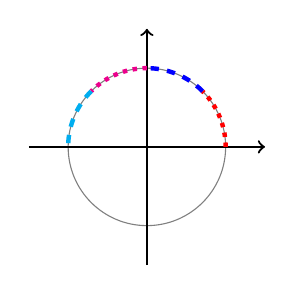
\begin{tikzpicture}
        [scale=1.,
        inner sep=0.5mm,
        pd/.style={circle,draw=red!50,fill=red!20,thick},
        hc/.style={circle,draw=blue!50,fill=blue!20,thick}]
        
        %draw unit circle
        \node (uni_circle1) at (0,0) {};
        \draw[black!50, thin] ($(uni_circle1)$) circle [radius=1];
        \draw[black, thick, ->] ($(uni_circle1)+(-1.5,0)$) -- ($(uni_circle1)+(1.5,0)$);%xaxis
        \draw[black, thick, ->] ($(uni_circle1)+(0,-1.5)$) -- ($(uni_circle1)+(0,1.5)$);%yaxis       

        \draw [dotted, ultra thick,red,domain=0:45] plot ({cos(\x)}, {sin(\x)});
        \draw [dashed, ultra thick,blue,domain=45:90] plot ({cos(\x)}, {sin(\x)});
        \draw [dotted, ultra thick,magenta,domain=90:135] plot ({cos(\x)}, {sin(\x)});
        \draw [dashed, ultra thick,cyan,domain=135:180] plot ({cos(\x)}, {sin(\x)});

        
    \end{tikzpicture}
\end{document}
